\section{Inverse Design for Elastostatics}
Given a set of base materials, an object layout, and functional objectives, the goal of our system is to compute the material distribution inside the object that optimizes the objectives.
In our approach, instead of computing per-voxel base material distribution, we work with microstructures made of the base materials and the space of physical material properties spanned by them. The complete pipeline of our system, illustrated in Figure \ref{fig:topoptOverview}, can be decomposed into two stages---gamut generation and gamut-constrained topology optimization.
\begin{figure}
	\centering
	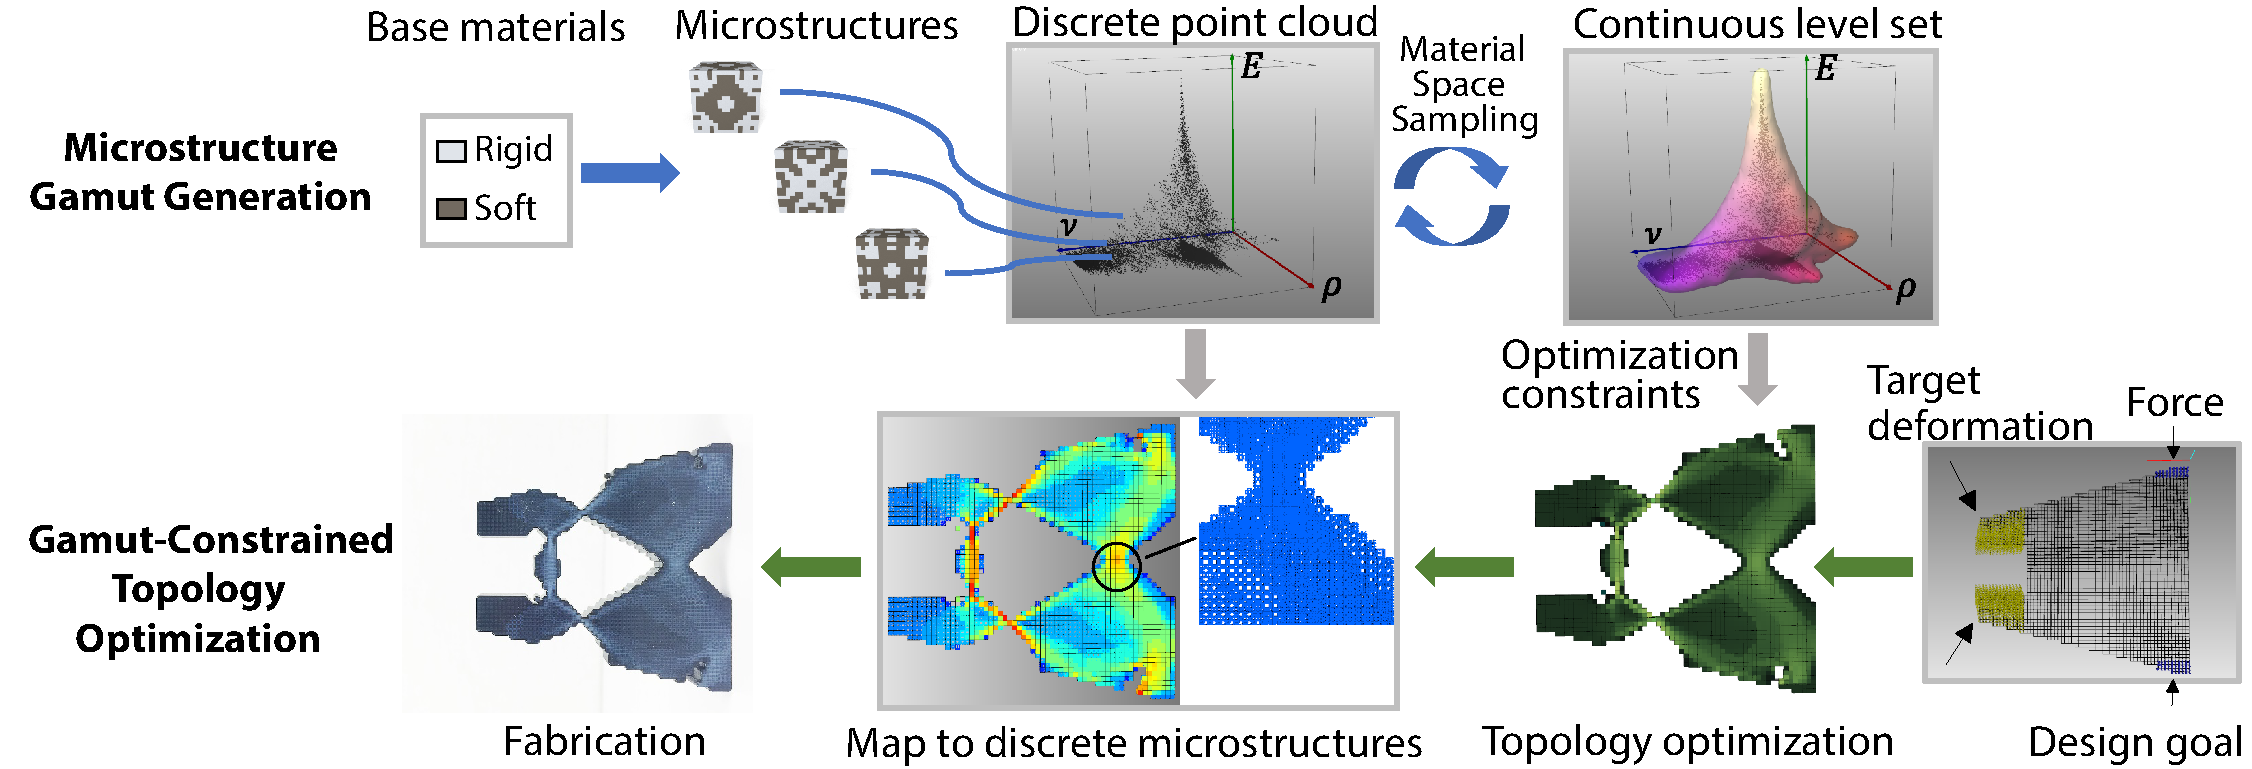
\includegraphics[width=0.95\textwidth]{images/topoptOverview.pdf}
	\caption{Inverse design algorithm.}
	\label{fig:topoptOverview}
\end{figure}
\paragraph{Gamut Generation}
In the first stage, we estimate the gamut of material properties covered by all possible microstructures made by spatial arrangement of base materials. 
Since exhaustively computing the properties of all these microstructures is, in practice, intractable, we progressively increase the material space by alternating a stochastic search and a continuous optimization. The first step introduces discrete changes in the materials of the microstructures and allows emergence of new types of microstructures. The second step allows to locally push the material space boundaries by refining the microstructure shapes. After completing this stage, we obtain a discrete representation of the space of material properties and the mapping between these properties and the corresponding microstructures.

\paragraph{Gamut-Constrained Topology Optimization}
In the second stage, we construct a smooth continuous gamut representation of the material property space by using a level set field. We define our topology optimization problem directly in this space. Our approach minimizes the objective function over possible material parameters while asking for strict satisfaction of the physics constraints -- typically, the static equilibrium -- as well as the strict satisfaction of the physical parameter bounds. Taking advantage of our gamut representation as a level set, we formulate this last constraint as limiting the material properties to stay on the negative side of the level set. This guarantees that the material properties that we use in the optimization are always physically realizable.
